% Created 2025-01-12 Sun 22:33
% Intended LaTeX compiler: pdflatex
\documentclass[presentation]{beamer}
\usepackage[utf8]{inputenc}
\usepackage[T1]{fontenc}
\usepackage{graphicx}
\usepackage{longtable}
\usepackage{wrapfig}
\usepackage{rotating}
\usepackage[normalem]{ulem}
\usepackage{amsmath}
\usepackage{amssymb}
\usepackage{capt-of}
\usepackage{hyperref}
\usepackage[T1]{fontenc}
\usepackage[utf8]{inputenc}
\usepackage[spanish]{babel}
\usepackage[backend=biber, style=apa]{biblatex}
\addbibresource{/home/juanubuntu/ArquitecturaCom/FormatoTareas/bibliography.bib}
\usetheme{default}
\usecolortheme{}
\usefonttheme{}
\useinnertheme{}
\useoutertheme{}
\author{Elizabeth Lopez, Francisco Morales, Juan Murillo}
\date{}
\title{S8-Buses-del-Sistema}

\hypersetup{
 pdfauthor={Elizabeth Lopez, Francisco Morales, Juan Murillo},
 pdftitle={S8-Buses-del-Sistema},
 pdfkeywords={},
 pdfsubject={},
 pdfcreator={Emacs 27.1 (Org mode 9.3)}, 
 pdflang={Spanish}}
\begin{document}

\maketitle
\begin{frame}{Outline}
\tableofcontents
\end{frame}



\section{Buses del Sistema (Sección)}
\label{sec:org24439da}
\begin{frame}[label={sec:org2dd0334}]{Estructuras de Interconexión (E1, 7, 97)}
\begin{itemize}
\item Conjunto de líneas que conectan los módulos elementales de un computador.
Para que se comuniquen e intercambien datos.
\item La estructura depende de los intercambios que se produzcan en los módulos.
\end{itemize}

\begin{center}
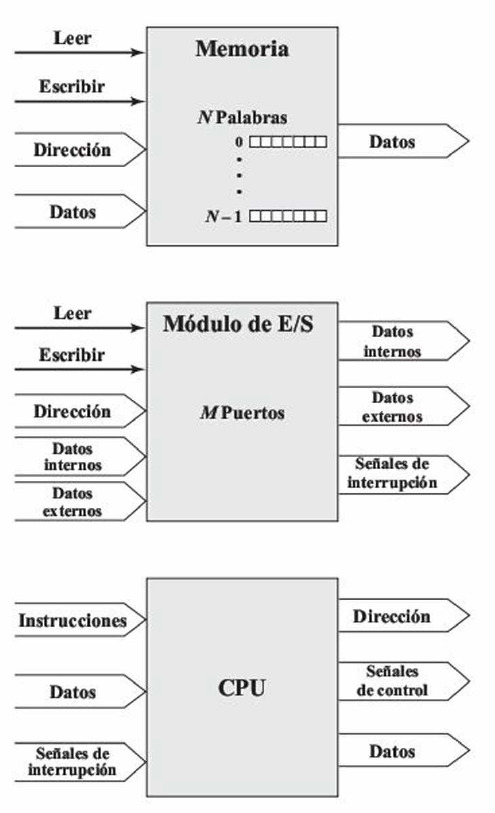
\includegraphics[width=0.3\textwidth]{./Images/Modulos.jpg}
\end{center}
\end{frame}

\begin{frame}[label={sec:org540a06e}]{Estructuras de Interconexión (E1, 7, 97)}
\alert{Módulos:}

\begin{itemize}
\item \alert{\alert{Memoria:}} constituido por N palabras de igual longitud. Se pueden realizar las
operaciones Read(Leer) y Write(Escribir). La posición de memoria se especifica
mediante una dirección.
\item \alert{\alert{Módulo de E/S:}} se encarga de controlar los dispositivos externos enlazados
a los puertos, donde se les asignara una dirección M. Controla los datos de salida
y entrada. Realiza las operaciones de lectura y escritura. Envía señales de interrupción.
\item \alert{\alert{Procesador:}} lee instrucciones y datos. Escribe datos después de procesarlos y
controla el funcionamiento del sistema. Puede recibir señales de interrupción.
\end{itemize}
\end{frame}

\begin{frame}[label={sec:orgd89c877}]{Estructuras de Interconexión (E1, 7, 97)}
\alert{Intercambios de Datos:}

\begin{itemize}
\item \alert{\alert{Memoria a procesador:}} el procesador lee información desde la memoria.
\item \alert{\alert{Procesador a memoria:}} el procesador escribe un dato en la memoria.
\item \alert{\alert{E/S a procesador:}} el procesador lee datos de un dispositivo de E/S.
\item \alert{\alert{Procesador a E/S:}} el procesador envía datos al dispositivo de  E/S.
\item \alert{\alert{Memoria a E/S - E/S a Memoria:}} ambos intercambian datos directamente.
\end{itemize}
\end{frame}

\section{Interconexión con Buses (Sección)}
\label{sec:org22d150a}
\begin{frame}[label={sec:org55b0111}]{Interconexión con Buses (E1, 7, 99)}
\begin{itemize}
\item Los buses son caminos de comunicación entre dos o más dispositivos con la
habilidad de transmitir señales hacia los demás o recibir las señales emitidas.
\item Solo un dispositivo puede emitir la señal en un periodo de tiempo. Si ambos
transmiten la señal, esta podria solaparse y distorsionarse.
\item Los caminos o lineas del bus transmiten señales binarias ya sea a travez de una
sola línea o de varias de manera paralela.
\item Existen diferentes tipos de buses para la comunicacion de diversos componentes.
El que trabaja con los módulos elementales se denomina (System bus).
\end{itemize}
\end{frame}

\begin{frame}[label={sec:orga6193ee}]{Estructura del Bus  (E1, 7, 99)}
\begin{center}
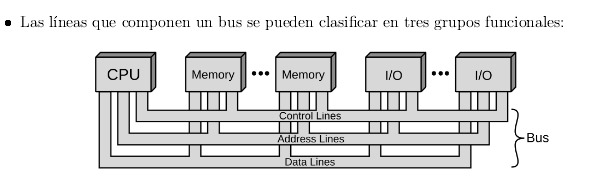
\includegraphics[width=0.8\textwidth]{./Images/Lineas.jpg}
\end{center}

\begin{itemize}
\item ¿Qué tipos de líneas componen un Bus de Sistema?
\begin{itemize}
\item Lineas de datos.
\item Lineas de direccion.
\item Lineas de control.
\end{itemize}
\end{itemize}
\end{frame}

\begin{frame}[label={sec:org17907c4}]{Estructura del Bus}
\begin{itemize}
\item ¿Qué son las líneas de datos?
\begin{itemize}
\item Transporte
\item Datos
\item Memoria -> Procesador
\end{itemize}
\end{itemize}
\end{frame}

\begin{frame}[label={sec:org1dc3831}]{Estructura del Bus}
\begin{itemize}
\item ¿Qué son las líneas de dirección?
\begin{itemize}
\item Ubicación
\item Memoria
\item Puertos de E/S
\item Anchura del bus
\end{itemize}
\end{itemize}
\end{frame}

\begin{frame}[label={sec:org8e2148c}]{Estructura del Bus}
\begin{itemize}
\item ¿Qué son las líneas de control?
\begin{itemize}
\item Control
\item Señales
\item Escritura
\item Lectura
\end{itemize}
\end{itemize}
\end{frame}

\begin{frame}[label={sec:org17bea74}]{Jerarquía de Buses Múltiples (E2, 7)}
Si se conecta un gran número de dispositivos al bus, las prestaciones pueden disminuir. Hay dos causas principales: 

\begin{enumerate}
\item Mayor retarde de propagación. Este retardo determina el tiempo que necesitan los dispositivos para coordinarse en el uso del bus.

\item Posible cuello de botella. Este problema se puede resolver en alguna medida incrementando la velocidad a la que el bus puede transferir los datos y utilizando buses más anchos (por ejemplo incrementando el bus de datos de 32 a 64 bits)
\end{enumerate}
\end{frame}
\begin{frame}[label={sec:org97cf9cb}]{Jerarquía de buses múltiples}
Por consiguiente, la mayoría de los computadores utilizan varios buses, normalmente organizados
jerárquicamente.

\begin{center}
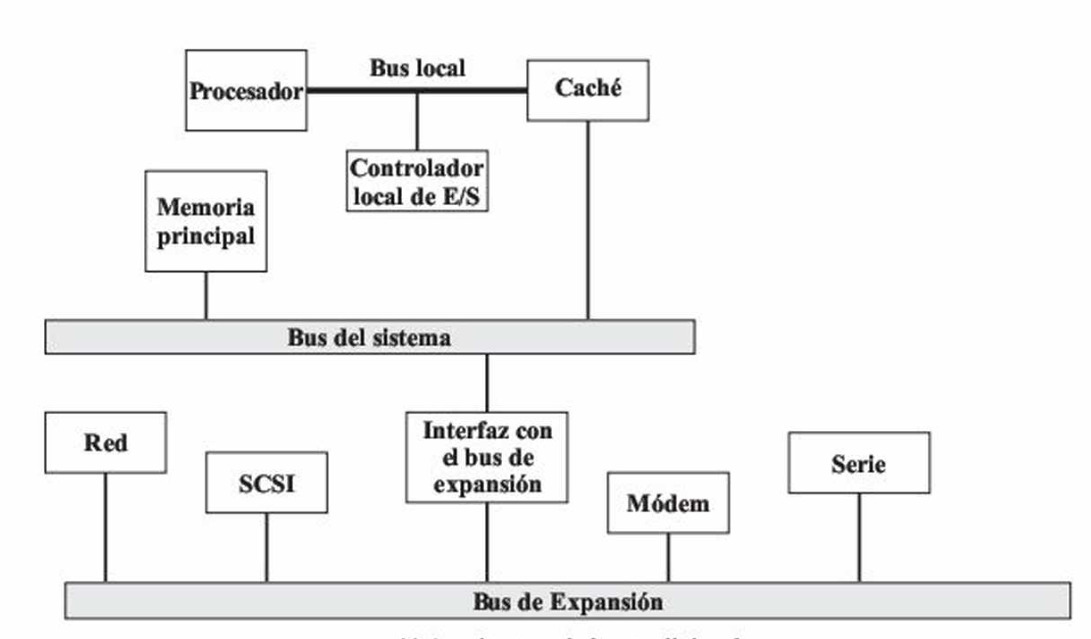
\includegraphics[width=0.8\textwidth]{./Images/jerarquiaBuses.jpeg}
\end{center} 
\end{frame}
\begin{frame}[label={sec:orgc7ce7ce}]{Jerarquía de buses múltiples}
La respuesta común a esta
situación, por parte de la industria, ha sido proponer un bus de alta velocidad que está estrechamente
integrado con el resto del sistema, y requiere solo un adaptador (bridge) entre el bus del procesador y
el bus de alta velocidad. En algunas ocasiones, esta disposición es conocida como arquitectura de
entreplanta (mezzanine architecture).

\begin{center}
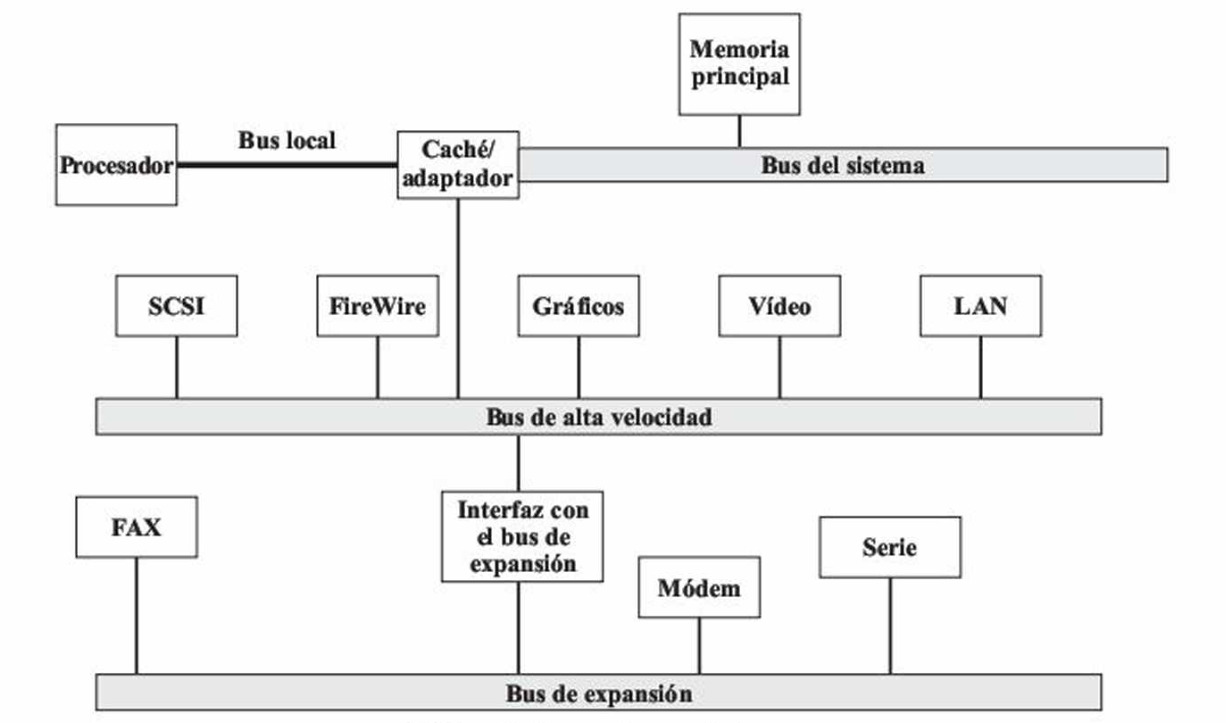
\includegraphics[width=0.8\textwidth]{./Images/jerarquiaBuses2.jpeg}
\end{center}
\end{frame}

\begin{frame}[label={sec:orgd104d9f}]{Jerarquía de buses múltiples}
La ventaja de esta organización es que el bus de alta velocidad acerca al procesador los dispositi
vos que exigen prestaciones elevadas y al mismo tiempo es independiente del procesador. Así, se pue
den tolerar las diferencias de velocidad entre el procesador y el bus de altas prestaciones y las
variaciones en la definición de las líneas de los buses. Los cambios en la arquitectura del procesador
no afectan al bus de alta velocidad, y viceversa.
\end{frame}
\begin{frame}[label={sec:org47502e5}]{Elementos de Diseño de un Bus (E2, 7)}
\end{frame}
\section{Interconexión punto a punto}
\label{sec:org34b8cbe}
\begin{frame}[label={sec:org83f7b79}]{Interconexión punto a punto}
La interconexión punto a punto consiste en establecer una conexión directa entre dos componentes de un sistema informáticos.
Esta arquitectura reemplazo a los buses compartidos, y la principal razón fue el aumento de frecuencia.

\begin{figure}[!h]
   \vspace{-0.1cm}
   \centering
   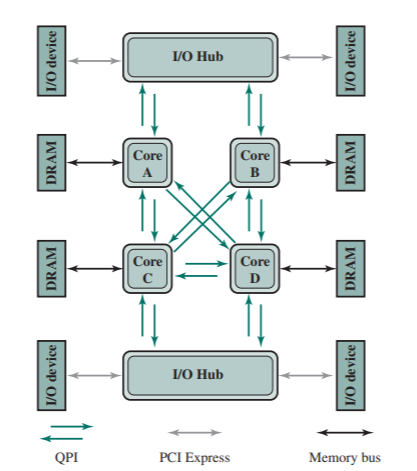
\includegraphics[height=4cm, width=0.8\textwidth]{./Images/image1.png}
   \vspace{-0.5cm} % Ajusta el espacio inferior
   \caption{Multiprocesador con QPIs}
   \label{fig:Representacion}
\end{figure}
\end{frame}

\begin{frame}[label={sec:orged4ec31}]{Ventajas}
\begin{columns}
\begin{column}{0.8\columnwidth}
\begin{itemize}
\item Elimina cuellos de botella asociados con buses compartidos.
\item Mejora la escalabilidad en sistemas multiprocesador, ya que cada procesador puede comunicarse con otros sin interferencias.
\item Aumenta la velocidad de transferencia y reduce la latencia.
\end{itemize}
\end{column}
\end{columns}
\end{frame}
\begin{frame}[label={sec:orgb74d3db}]{QPI (E3, 11)}
\end{frame}
\section{PCI Express (E4, 11)}
\label{sec:orgbf211cc}
\begin{frame}[label={sec:orgb9a1c11}]{PCI Express (E4, 11)}
\end{frame}
\section{Referencias}
\label{sec:org173474d}
\begin{frame}[allowframebreaks]{Bibliografía}
\printbibliography
\end{frame}
\end{document}
